%%%%%%%%%%%%%%%%%%%%%%%%%%%%%%%%%%%%%%%%%%%%%%%%%%%%%%%%%%%
%% Principios del diseño

\section{Visión general del desarrollo y principios del diseño técnico.}\label{principios:vision-general-desarrollo}

\subsection{Principios de diseño TDD.}\label{principios:principios-de-diseno}
Se pretende generar un código sólido, flexible y eficiente; pero el énfasis en esta primera etapa de desarrollo, será hacia la \emph{flexibilidad}. En principio, la idea original de diseño es solo eso, una idea. A medida que se vaya obteniendo más información y \emph{aprendamos más del proceso de desarrollo y los requerimientos del diseño}, deberemos ir refactorizando el código (reestructurar su estructura interna sin alterar su comportamiento externo) para obtener unidades más definidas y alineadas a los requerimientos, pero sobretodo unidades más fáciles de mantener.

Para esto se deberá implementar un sistema de pruebas para cada feature que se trabaje. Esto implica invertir el proceso de desarrollo escribiendo primero el test, dejar que falle y a continuación implementar la funcionalidad. El principio es concentrarse en las pruebas no en el \foreignlanguage{english}{debugging}; aunque es ineludible, \emph{no queremos estar arreglando bugs, sino que queremos evitarlos}.

Se simplifica el diseño para agilizar el desarrollo y facilitar el mantenimiento.

\subsection{Desarrollo dirigido por tests (TDD).}\label{principios:TDD}

\begin{figure}[ht]
	\centering
	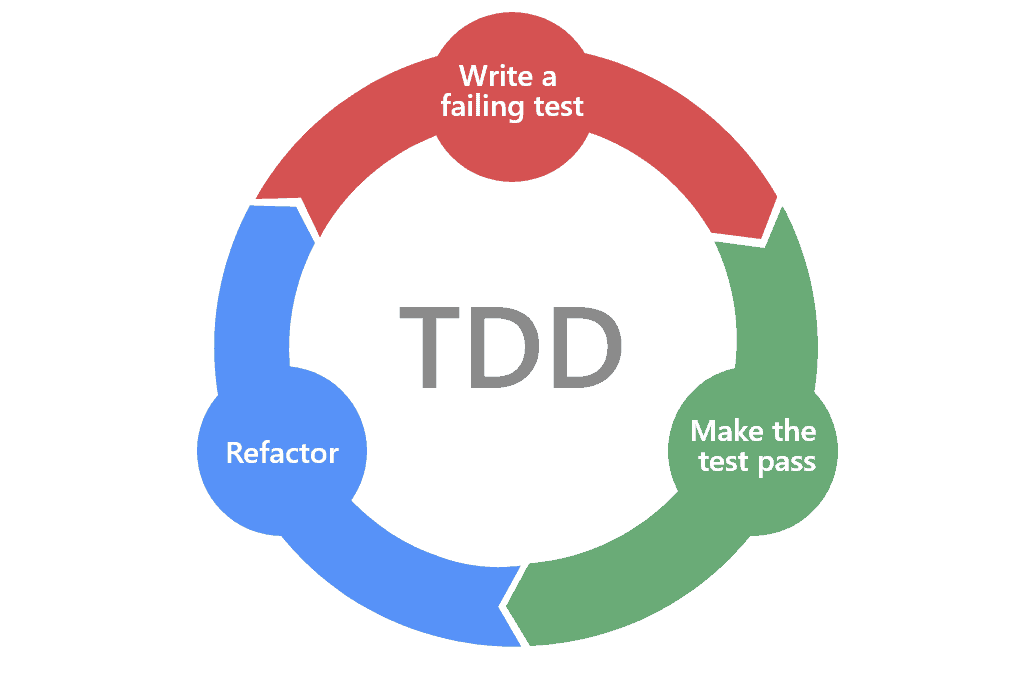
\includegraphics[width=0.75\textwidth]{imágenes/tdd.png}
	\caption{Flujo de desarrollo TDD.}
\end{figure}

Se comienza a trabajar por la fase roja escribiendo un test que supervise la implementación de la nueva funcionalidad. \emph{No queremos probar cómo funciona el código, sino probar que se comporte de la forma que esperamos}. Dado que aún el código no ha sido implementado este test fallará (muy importante que el test falle).

A continuación en la fase verde, se trabaja en la implementación del código tratando de superar el test de la forma más directa y rápida posible; \textit{no importa que el código sea horrible}.

Habiendo superado el test sabemos que contamos con un código que funciona, por lo mismo pasamos a la fase azul donde refactorizamos este código ahora en búsqueda de eficiencia y limpieza. Ya que contamos con nuestros test unitarios, podremos saber en todo momento cuando nuestra refactorización es correcta o genera problemas.

Repetimos el ciclo hasta alcanzar nuestras metas de implementación.

Cumpliendo esta metodología, se otorgará mayor flexibilidad para el diseño creativo del juego. Al mismo tiempo, dada la magnitud y complejidad de todo el sistema, ya que el testeo del código es parte del proceso de desarrollo se pretende minimizar considerablemente la cantidad de bugs que llegue a la rama \textbf{main} (ver el apartado \nameref{flujo:repositorio}).

\subsection{Refactorización: Rendimiento y limpieza.}\label{principios:refactorizacion-rendimiento-limpieza}
Aunque es frecuente limpiar el código a medida que se escribe, al hacer eso no estamos refactorizando; el factor clave de la refactorización es hacerlo intencionalmente pero de forma separada a la adición de nueva funcionalidad. \emph{Al ya tener definidas las pruebas, la reescritura del código se puede hacer con seguridad y confianza}.

El objetivo en este proceso es doble, por un lado se busca un rendimiento óptimo en los apartados que lo requieran (combate, IA, físicas y animación por ejemplo) y por otro la revisión del código además de mejorar la legibilidad del mismo (mejores nombres de funciones, variables y comentarios), nos ayuda al entendimiento del sistema y puede señalar oportunidades de encapsulación y mejoras al modelamiento.

\subsubsection{Documentación dentro del código.}\label{principios:documentacion-en-codigo}
La búsqueda de simplicidad en el diseño también aplica a la documentación del código. Idealmente éste debe estar “autodocumentado”, es decir que los nombres de las variables, métodos y clases den cuenta de manera transparente e intuitiva su rol dentro de la lógica. Al mismo tiempo en los casos más complejos es de vital importancia añadir comentarios no solo para facilitar la comprensión del sentido de ciertas líneas especialmente oscuras, sino para ayudar al futuro proceso de refactorización y debbuging. \emph{Los nombres largos no lastran la eficiencia del código}.

En cuanto al formato del código, dado que \lsc{GDS}cript está basado en Python, además de las propias sugerencias de Godot se recomienda seguir la \href{https://www.python.org/dev/peps/pep-0008/}{guía de estilo PEP-8}. En especial las referidas al límite horizontal de 79 carácteres, separación entre funciones de 1 línea en blanco y 2 entre clases, la indentación por 4 espacios, y operadores y variables separados por un espacio (ej: {\small \texttt{var direction = Vector2(2, 5 + PI)}}).

Aplicando simplicidad junto al desarrollo colectivo del software nos aseguramos que a medida que el código crezca, el equipo conocerá de mejor manera y con mayor amplitud el sistema completo y sus interacciones.


